% GNUPLOT: LaTeX picture with Postscript
\begingroup
  \makeatletter
  \providecommand\color[2][]{%
    \GenericError{(gnuplot) \space\space\space\@spaces}{%
      Package color not loaded in conjunction with
      terminal option `colourtext'%
    }{See the gnuplot documentation for explanation.%
    }{Either use 'blacktext' in gnuplot or load the package
      color.sty in LaTeX.}%
    \renewcommand\color[2][]{}%
  }%
  \providecommand\includegraphics[2][]{%
    \GenericError{(gnuplot) \space\space\space\@spaces}{%
      Package graphicx or graphics not loaded%
    }{See the gnuplot documentation for explanation.%
    }{The gnuplot epslatex terminal needs graphicx.sty or graphics.sty.}%
    \renewcommand\includegraphics[2][]{}%
  }%
  \providecommand\rotatebox[2]{#2}%
  \@ifundefined{ifGPcolor}{%
    \newif\ifGPcolor
    \GPcolortrue
  }{}%
  \@ifundefined{ifGPblacktext}{%
    \newif\ifGPblacktext
    \GPblacktextfalse
  }{}%
  % define a \g@addto@macro without @ in the name:
  \let\gplgaddtomacro\g@addto@macro
  % define empty templates for all commands taking text:
  \gdef\gplbacktext{}%
  \gdef\gplfronttext{}%
  \makeatother
  \ifGPblacktext
    % no textcolor at all
    \def\colorrgb#1{}%
    \def\colorgray#1{}%
  \else
    % gray or color?
    \ifGPcolor
      \def\colorrgb#1{\color[rgb]{#1}}%
      \def\colorgray#1{\color[gray]{#1}}%
      \expandafter\def\csname LTw\endcsname{\color{white}}%
      \expandafter\def\csname LTb\endcsname{\color{black}}%
      \expandafter\def\csname LTa\endcsname{\color{black}}%
      \expandafter\def\csname LT0\endcsname{\color[rgb]{1,0,0}}%
      \expandafter\def\csname LT1\endcsname{\color[rgb]{0,1,0}}%
      \expandafter\def\csname LT2\endcsname{\color[rgb]{0,0,1}}%
      \expandafter\def\csname LT3\endcsname{\color[rgb]{1,0,1}}%
      \expandafter\def\csname LT4\endcsname{\color[rgb]{0,1,1}}%
      \expandafter\def\csname LT5\endcsname{\color[rgb]{1,1,0}}%
      \expandafter\def\csname LT6\endcsname{\color[rgb]{0,0,0}}%
      \expandafter\def\csname LT7\endcsname{\color[rgb]{1,0.3,0}}%
      \expandafter\def\csname LT8\endcsname{\color[rgb]{0.5,0.5,0.5}}%
    \else
      % gray
      \def\colorrgb#1{\color{black}}%
      \def\colorgray#1{\color[gray]{#1}}%
      \expandafter\def\csname LTw\endcsname{\color{white}}%
      \expandafter\def\csname LTb\endcsname{\color{black}}%
      \expandafter\def\csname LTa\endcsname{\color{black}}%
      \expandafter\def\csname LT0\endcsname{\color{black}}%
      \expandafter\def\csname LT1\endcsname{\color{black}}%
      \expandafter\def\csname LT2\endcsname{\color{black}}%
      \expandafter\def\csname LT3\endcsname{\color{black}}%
      \expandafter\def\csname LT4\endcsname{\color{black}}%
      \expandafter\def\csname LT5\endcsname{\color{black}}%
      \expandafter\def\csname LT6\endcsname{\color{black}}%
      \expandafter\def\csname LT7\endcsname{\color{black}}%
      \expandafter\def\csname LT8\endcsname{\color{black}}%
    \fi
  \fi
  \setlength{\unitlength}{0.0500bp}%
  \begin{picture}(7200.00,5040.00)%
    \gplgaddtomacro\gplbacktext{%
      \csname LTb\endcsname%
      \put(1100,1018){\makebox(0,0)[r]{\strut{} 5000}}%
      \put(1100,1438){\makebox(0,0)[r]{\strut{} 10000}}%
      \put(1100,1858){\makebox(0,0)[r]{\strut{} 15000}}%
      \put(1100,2278){\makebox(0,0)[r]{\strut{} 20000}}%
      \put(1100,2698){\makebox(0,0)[r]{\strut{} 25000}}%
      \put(1100,3119){\makebox(0,0)[r]{\strut{} 30000}}%
      \put(1100,3539){\makebox(0,0)[r]{\strut{} 35000}}%
      \put(1100,3959){\makebox(0,0)[r]{\strut{} 40000}}%
      \put(1100,4379){\makebox(0,0)[r]{\strut{} 45000}}%
      \put(1100,4799){\makebox(0,0)[r]{\strut{} 50000}}%
      \put(1220,440){\makebox(0,0){\strut{} 0}}%
      \put(2023,440){\makebox(0,0){\strut{} 20}}%
      \put(2825,440){\makebox(0,0){\strut{} 40}}%
      \put(3628,440){\makebox(0,0){\strut{} 60}}%
      \put(4431,440){\makebox(0,0){\strut{} 80}}%
      \put(5234,440){\makebox(0,0){\strut{} 100}}%
      \put(6036,440){\makebox(0,0){\strut{} 120}}%
      \put(6839,440){\makebox(0,0){\strut{} 140}}%
      \put(160,2719){\rotatebox{-270}{\makebox(0,0){\strut{}Energia Consumida (J)}}}%
      \put(4029,140){\makebox(0,0){\strut{}Tempo de Simulação (s)}}%
    }%
    \gplgaddtomacro\gplfronttext{%
      \csname LTb\endcsname%
      \put(3860,4636){\makebox(0,0)[r]{\strut{}Consumo por Intervalo}}%
      \csname LTb\endcsname%
      \put(3860,4436){\makebox(0,0)[r]{\strut{}Energia Acumulada}}%
    }%
    \gplbacktext
    \put(0,0){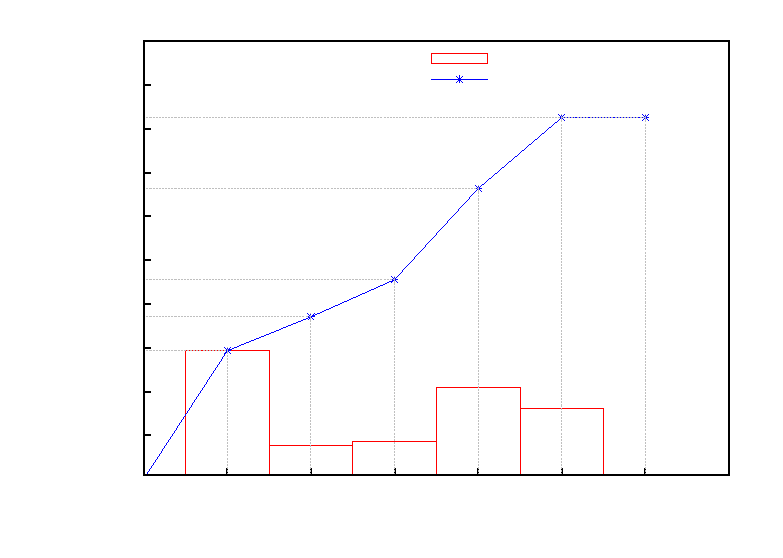
\includegraphics{./images/s1-partial-approx-v}}%
    \gplfronttext
  \end{picture}%
\endgroup
